\section{Overall description}
Here you can see how to include an image in your document.

\begin{sidewaysfigure}
\centering
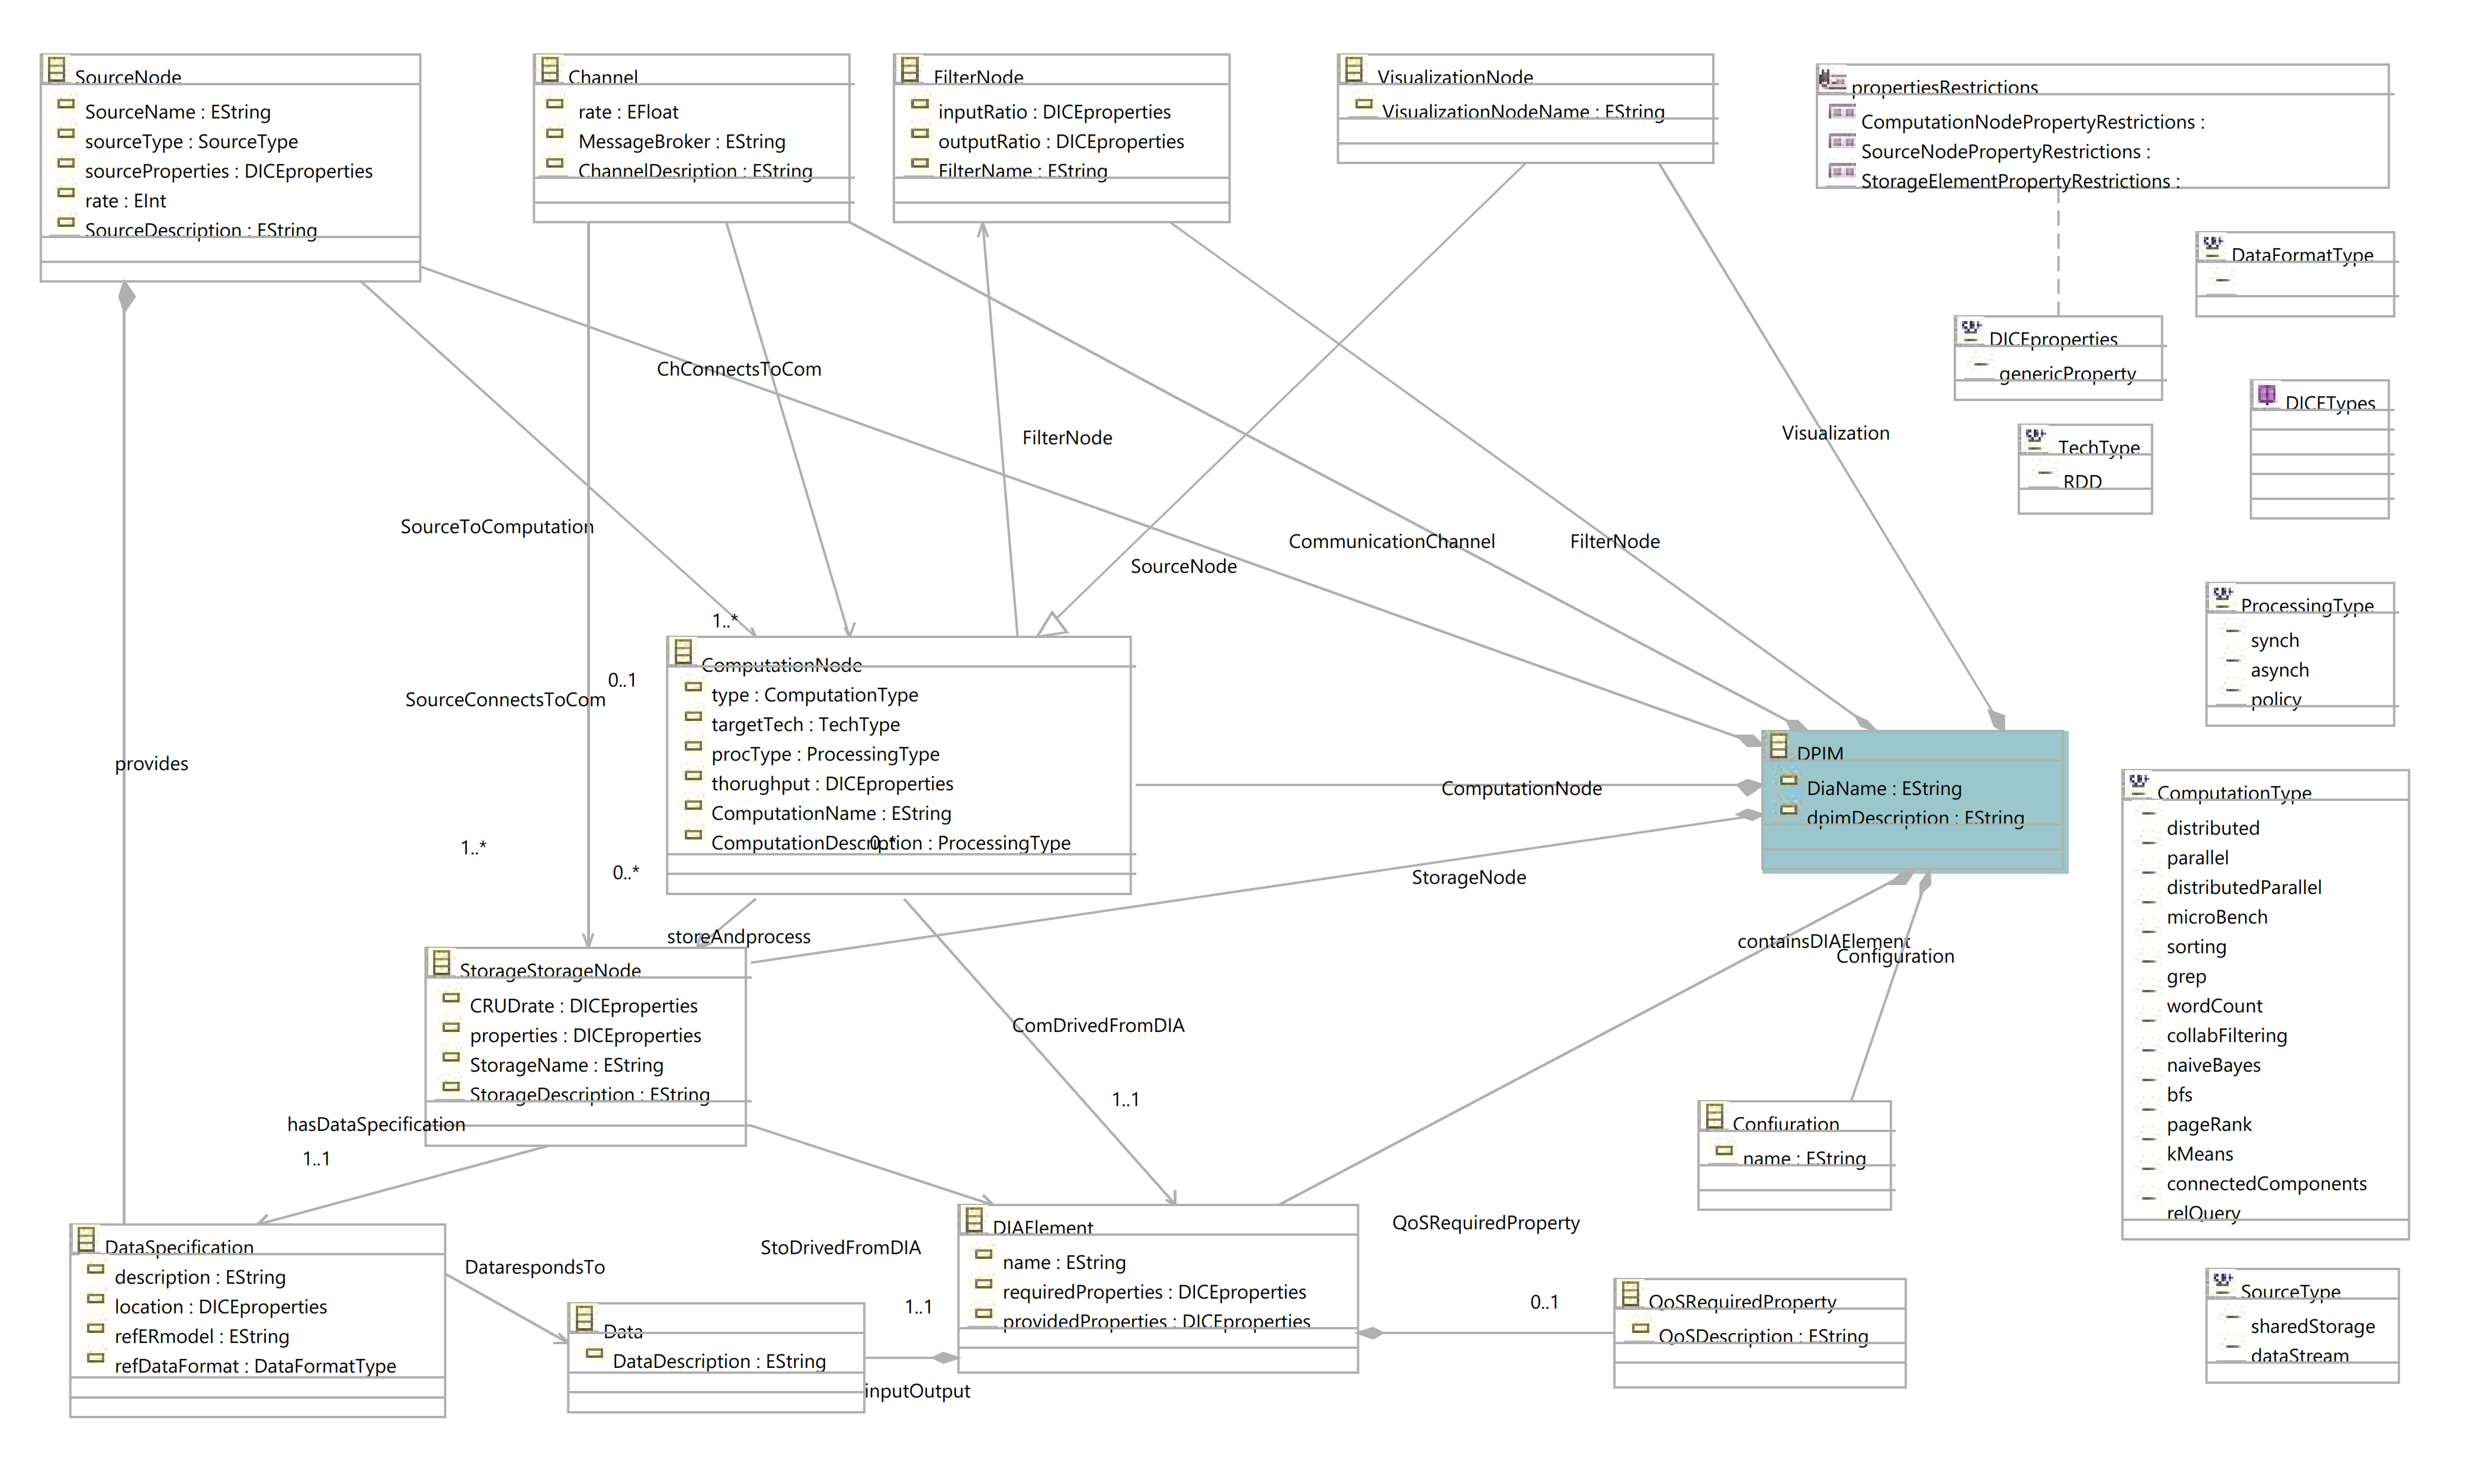
\includegraphics[width=\textwidth]{Images/11.png}
\caption{\label{fig:metamodel}DICE DPIM metamodel.}
\end{sidewaysfigure}

\begin{figure}
\centering
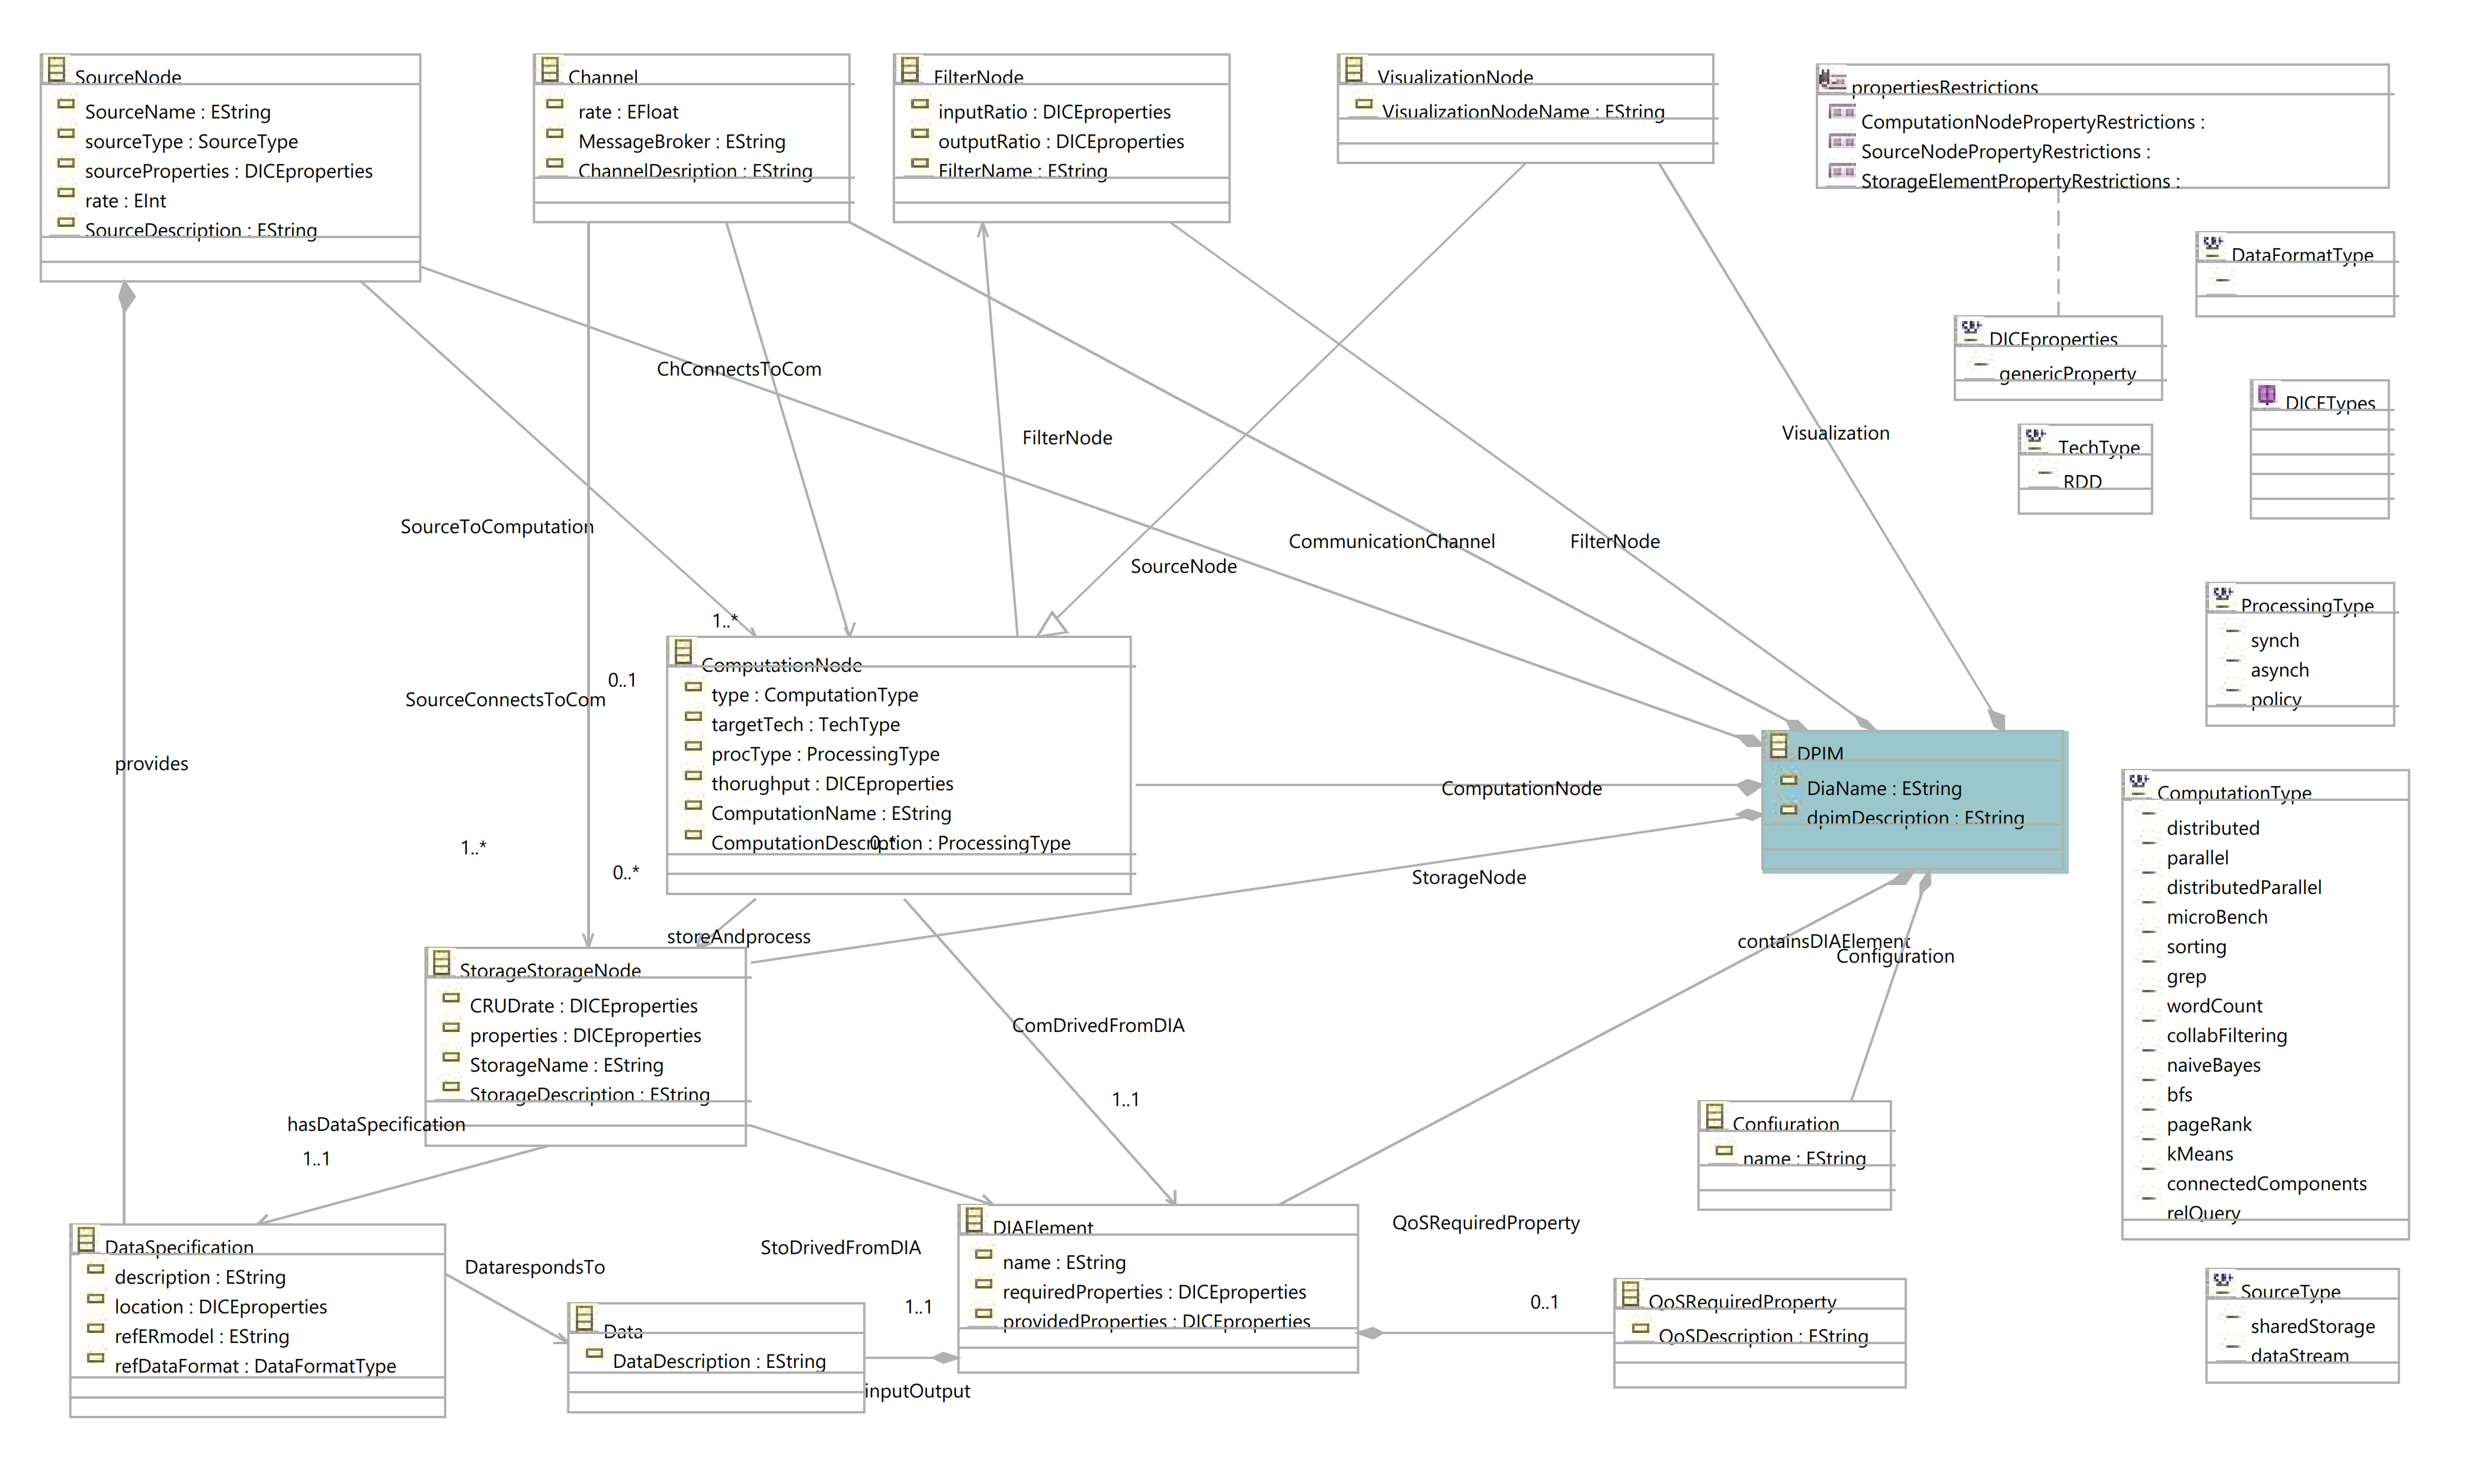
\includegraphics[width=\textwidth]{Images/11.png}
\caption{\label{fig:metamodel2}DICE DPIM metamodel in portrait form.}
\end{figure}

\subsection{Product perspective}
\subsubsection{scenarios}
\subsubsection{further details on shared phenomena}
\subsubsection{domain model: class diagrams and statecharts}
\subsection{Product functions}
most important requirements
\subsection{User characteristics}
\subsubsection{Actors}

Customer: a person who grocery shops.}
Unregistered user: a customer using CLup without being registered. They can join the virtual queue and ask/receive updates.}
Registered user/User: a customer using Clup and who is registered on the system. They can join the virtual queue, book a shopping session and ask/receive updates.}
Shop manager: a person who register their shop on Clup. A shop manager can register multiple shop on the system.}
Shop: a grocery shop registered on the system. It updates periodically the people present in the store and sends updates to the manager.}


\subsection{Assumptions, dependencies and constraints}
\subsubsection{Domain Assumptions}

